\subsection{An\'{a}lise Relacionada à Primeira Questão de Pesquisa}

\begin{enumerate}[(QP1)]

\item O que caracteriza a modernização dos sistemas legados de 
acordo com a literatura existente? Quais outros termos estão relacionados 
com a modernização?

\end{enumerate}

Para responder essa questão, buscou-se caracterizar a modernização dos sistemas 
legados no contexto da manutenção de software. Assim, como pode-se 
verificar em~\cite{S01_bennett2000software, S9_bianchi:2003, S3_Bisbal:1999, S15_Comella-DordaASurvey2000, S2_erlikh:2000}, 
a modernização pode ser caracterizada pela necessidade de evolução dos sistemas para adequá-lo aos requisitos de negócio das organizações, 
seja com novas funcionalidades, correção de erros ou atualizações tecnológicas. Nesse sentido, muitas teorias 
tem sido sugeridas na literatura, como discutido a seguir. 

\textbf{N. Weiderman et al.} introduzem um modelo de ciclo de vida 
para descrever a evolução de um sistema durante a sua vida útil~\cite{S15_Comella-DordaASurvey2000, Seacord:2003, S12_WeidermanApproaches:1997}. 
Neste modelo, existem três fases distintas: manutenção, modernização e substituição. Durante o ciclo de vida de um sistema, pequenas 
modificações são realizadas através das manutenções para satisfazer algum requisito ou corrigir algum erro. As mudanças de maior impacto, 
como requisitos de negócios importantes, mudanças na arquitetura do sistema ou a migração do sistema para outra plataforma são realizadas na fase 
de modernização. Todavia, quando o sistema torna-se muito resistente para evoluir por alguma razão específica, este é substituído. 
Nesse ciclo, as necessidades de negócio da organização são intercaladas com as implementações realizadas para suprir essas necessidades. 
Além de introduzir um modelo de ciclo de vida, Weiderman também propõem distinguir a modernização pelo nível de compreensão requerido para suportar 
os esforços de modernização: \textit{White-box} para compreensão das estruturas internas do sistemas e \textit{Black-box} quando requer somente a compreensão das interfaces externas dos sistemas legados.

\textbf{K. Bennett et al.} propõem um modelo chamado 
\textit{staged model} para descrever o ciclo de vida de um sistema e auxiliar na identificação das principais 
áreas de pesquisa sobre modernização~\cite{S01_bennett2000software}. Este modelo divide-se em 5 etapas: 
\textit{initial development, evolution, servicing, phase-out, close-down}. Aqui, a modernização compreende a fase \textit{evolution} e, 
ao contrário do modelo proposto por Weiderman et al., é considerada uma atividade de manutenção, que pode ser classificada em 
4 classes: adaptativa, quando há alterações no ambiente do software; perfectiva, para novos requerimentos do usuário; corretiva, correção de erros; e preventiva, para 
prevenir problemas futuros. 

\textbf{J. Bisbal et al.} apresentam um modelo de ciclo de vida, onde o foco são as atividades evolutivas ordenadas pelo impacto causado nos 
sistemas~\cite{S3_Bisbal:1999}. Assim, dividem-se em \textit{wrapping}, cujo objetivo é prover uma nova interface para os componentes de um sistema, 
tornando-os mais acessíveis para outros componentes; manutenção, para os pequenos ajustes e correção de erros; a migração, que visa mover o sistema 
legado para um ambiente mais flexível, mantendo os dados e funcionalidades originais; e o redesenvolvimento, que reescreve por completo as aplicações. 

Percebe-se que, embora esses modelos usem termos distintos para referir-se as fases do ciclo de vida dos sistemas, há várias semelhanças. Por exemplo, 
o significado de substituição é o mesmo que redesenvolvimento e o significado de migração é o mesmo que modernização. No entanto, 
a fase \textit{wrapping} descrita por Bisbal et al. é uma técnica de modernização \textit{Black-box} em Weiderman.

Prosseguindo com esta análise, tendo em vista à diversidade de termos para referir-se as abordagens de modernização, 
para responder as demais questões de pesquisa, optou-se pelo modelo proposto por Weiderman et al.. Sendo assim, segue um breve resumo de cada 
fase neste modelo evolutivo:

\begin{description}

\item[Manutenção] é a primeira fase do ciclo de vida de um sistema. Ela inicia tão logo o sistema entra em produção, 
sendo considerado um processo iterativo e incremental, através do qual, pequenas modificações são aplicadas ao sistema, 
de maneira pontual e localizada~\cite{S01_bennett2000software, S12_WeidermanApproaches:1997}. No entanto, como salienta~\cite{Seacord:2003}, 
essas modificações atendem as necessidades das organizações apenas por um determinado período, deteriorando-se posteriormente.

\item[Modernização] ocorre quando a manutenção não é suficiente para manter o sistema atualizado e alinhado aos objetivos de negócios. 
Segundo~\cite{S01_bennett2000software, S3_Bisbal:1999, S12_WeidermanApproaches:1997}, compreendem alterações maiores, como por exemplo, a implementação de um requisito importante, 
mudanças na arquitetura ou migração do sistema para uma nova plataforma. Assim, como observado em~\cite{S01_bennett2000software}, a modernização é mais pervasiva que a manutenção, 
sendo um dos principais aspectos que os diferenciam. Por fim, conforme salienta~\cite{Seacord:2003}, a modernização deve preservar as funcionalidades e os dados do sistema, caso contrário, 
representaria uma substituição. 

\item[Substituição] fase também conhecida como \textit{Big Bang} ou \textit{Cold Turkey}~\cite{Seacord:2003}, normalmente é utilizada quando o sistema 
legado torna-se muito resistente e inflexível para ser modernizado, não há documentação ou o custo de manutenção não compensa mais~\cite{S01_bennett2000software, S3_Bisbal:1999, S12_WeidermanApproaches:1997}.

\end{description}

Com este breve resumo das características de cada fase do ciclo de vida de um sistema, finaliza-se a questão QP1 com um \textit{word cloud} 
dos 30 termos mais citados nos \textit{abstracts} das fontes primárias selecionadas. Esses termos podem ser visualizados na 
Figura~\ref{fig:word_cloud}. Note que, sob a perspectiva tecnol\'{o}gica, \'{e} poss\'{i}vel perceber nessa figura um certo grau de 
interesse na computa\c c\~{a}o orientada a servi\c cos. 


\begin{figure}[ht]
\centering
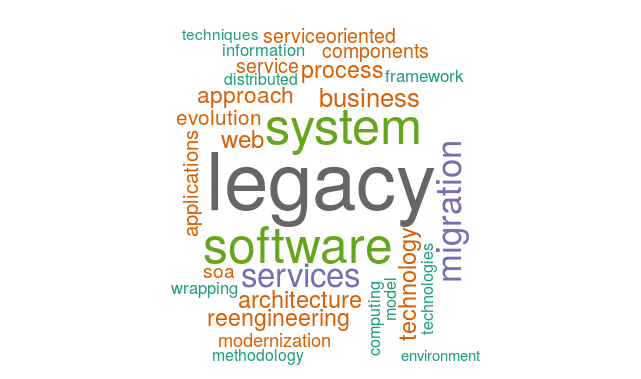
\includegraphics[scale=0.40]{img/mapeamento/word_cloud.png}
\caption{Termos mais citados nos \textit{abstracts} das fontes primárias selecionadas.}
\label{fig:word_cloud}
\end{figure}
